\chapter{Background}
% NOTE: Assume that the reader has common computer science knowledge!
In this chapter we are introducing knowledge which is required to understand the content of this thesis.
In \cref{sec:bg:compilers} we give an overview about how a compiler is typically implemented and which problems it has to solve that we want to tackle.
The \crefrange{sec:bg:compilers:frontend}{sec:bg:compilers:optimizer} give a superficial overview of the first two phases of a typical compiler.
\Cref{sec:bg:compilers:backend} gives a more detailed introduction to compiler back ends, which we aim to optimize in this thesis.
\todo{explain also the other sections}

%\section{Motivation?}
%\cite{goodman1988code} state the important interdependence between instruction scheduling and register allocation.

\section{CPU Functionality}
\label{sec:bg:cpu}


\begin{figure}
    \centering

    % TODO: move these definitions somewhere else?
    \definecolor{darkgray}{HTML}{3D4752}
    \tikzstyle{instr} = [rectangle, rounded corners, minimum width=3cm, minimum height=1cm,text centered, text=white, fill=darkgray]
    \tikzstyle{arrow} = [thick,->,>=stealth]
    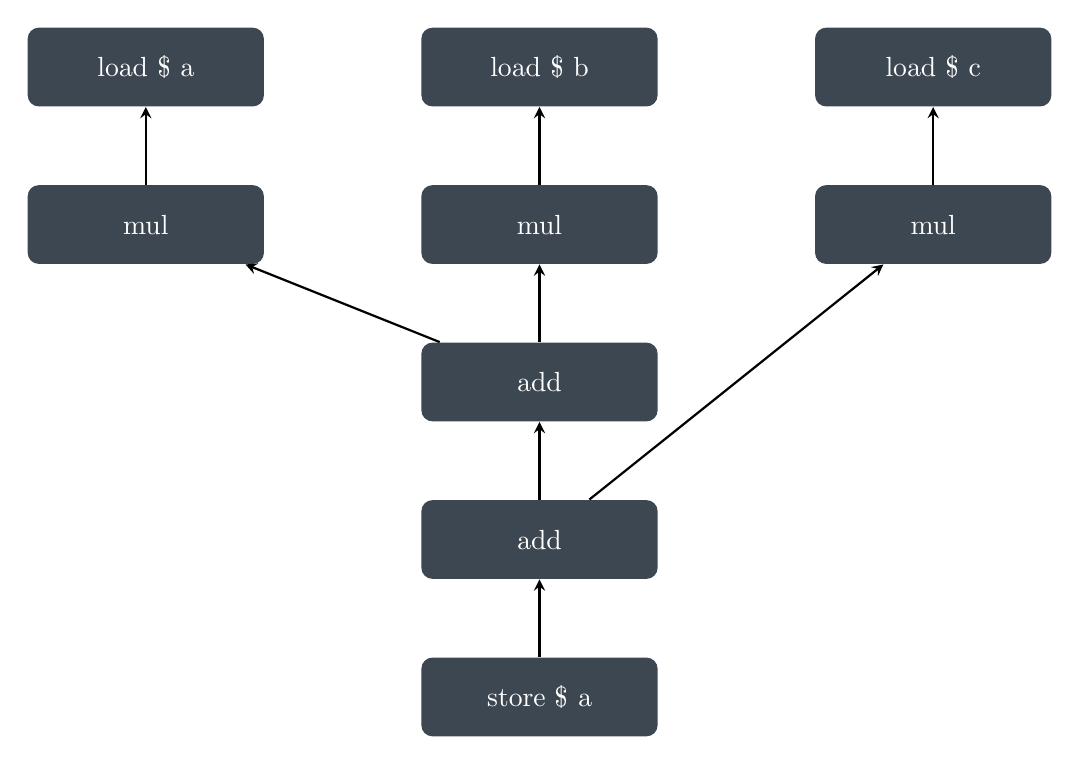
\begin{tikzpicture}[node distance=2cm]
        \node (load_a) [instr] {\lstinline{load \$ a}};
        \node (mul_a_a) [instr, below of=load_a] {\lstinline{mul}};
        \node (load_b) [instr, right of=load_a, xshift=3cm] {\lstinline{load \$ b}};
        \node (mul_b_b) [instr, below of=load_b] {\lstinline{mul}};
        \node (load_c) [instr, right of=load_b, xshift=3cm] {\lstinline{load \$ c}};
        \node (mul_c_c) [instr, below of=load_c] {\lstinline{mul}};
        \node (add_a_b) [instr, below of=mul_b_b] {\lstinline{add}};
        \node (add_ab_c) [instr, below of=add_a_b] {\lstinline{add}};
        \node (store) [instr, below of=add_ab_c] {\lstinline{store \$ a}};
        
        \draw [arrow] (mul_a_a) -- (load_a);
        \draw [arrow] (mul_b_b) -- (load_b);
        \draw [arrow] (mul_c_c) -- (load_c);
        \draw [arrow] (add_a_b) -- (mul_a_a);
        \draw [arrow] (add_a_b) -- (mul_b_b);
        \draw [arrow] (add_ab_c) -- (add_a_b);
        \draw [arrow] (add_ab_c) -- (mul_c_c);
        \draw [arrow] (store) -- (add_ab_c);    
    \end{tikzpicture}
    \caption{Example DAG a=a*a+b*b+c*c}
    \label{fig:example_dag}
\end{figure}

% \begin{table}
%     \centering
%     \begin{tabular}{cclcl} 
%         \toprule
%         Start & Occupied & \multicolumn{3}{l}{Instruction} \\
%         Cycle &  Cycles &&&\\
%         \midrule
%         1  & 1-3   & \lstinline{load \$ a}  & \rightarrow & \lstinline{a} \\
%         4  & 4-5   & \lstinline{mul a, a} & \rightarrow & \lstinline{a} \\
%         5  & 5-7   & \lstinline{load \$ b}  & \rightarrow & \lstinline{b} \\
%         8  & 8-9   & \lstinline{mul b, b} & \rightarrow & \lstinline{b} \\
%         9  & 9-11  & \lstinline{load \$ c}  & \rightarrow & \lstinline{c} \\
%         12 & 12-13 & \lstinline{mul c, c} & \rightarrow & \lstinline{c} \\
%         13 & 13    & \lstinline{add a, b} & \rightarrow & \lstinline{a} \\
%         14 & 14    & \lstinline{add a, c} & \rightarrow & \lstinline{a} \\
%         15 & 15-17 & \lstinline{store a}  & \rightarrow & \lstinline{\$ a} \\
%         \bottomrule
%     \end{tabular}
%     \caption{Unscheduled example \lstinline{a=a*a+b*b+c*c}}
%     \label{table:1}
% \end{table}

% \begin{table}
%     \centering
%     \begin{tabular}{cclcl} 
%         \toprule
%         Start & Occupied & \multicolumn{3}{l}{Instruction} \\
%         Cycle &  Cycles &&&\\
%         \midrule
%         1 & 1-3  & \lstinline{load \$ a}  & \rightarrow & \lstinline{a} \\
%         2 & 2-4  & \lstinline{load \$ b}  & \rightarrow & \lstinline{b} \\
%         3 & 3-5  & \lstinline{load \$ c}  & \rightarrow & \lstinline{c} \\
%         4 & 4-5  & \lstinline{mul a, a} & \rightarrow & \lstinline{a} \\
%         5 & 5-6  & \lstinline{mul b, b} & \rightarrow & \lstinline{b} \\
%         6 & 6-7  & \lstinline{mul c, c} & \rightarrow & \lstinline{c} \\
%         7 & 7    & \lstinline{add a, b} & \rightarrow & \lstinline{a} \\
%         8 & 8    & \lstinline{add a, c} & \rightarrow & \lstinline{a} \\
%         9 & 9-11 & \lstinline{store a}  & \rightarrow & \lstinline{\$ a} \\
%         \bottomrule
%     \end{tabular}
%     \caption{Scheduled example \lstinline{a=a*a+b*b+c*c}}
%     \label{table:2}
% \end{table}

ISA\\
Memory and Registers\\
How do CPUs work in general? -> Fetch, Decode, etc.\\
In-order vs out-of-order architectures

\section{Compilers}
\label{sec:bg:compilers}
%What is a compiler? \\
% \todo{This is probably too basic and not required. Might maybe be used in introduction, though}
% In the early days of computer programming, computers were programmed in assembly languages.
% These languages are exclusive to specific processor architectures and only provide the instructions that are available by the \ac{isa} of the processor.
% This approach has several disadvantages.
% Lots of complicated code, that is hard to understand, is written to express even simple programs.
% Also, each program has to be rewritten to execute on a processor with another architecture.
%
% Nowadays computers are programmed---almost exclusively---in high-level programming languages like C/C++, Java, Python, etc.
% The processor is not able to execute code written in such high-level programming languages, though.
% For this reason a compiler has to translate the code into a format that the processor can understand.
Making computer programs, that are written in high-level programming languages~(\eg C/C++, Java, Rust), executable on a specific machine is not a trivial task.
Compilers are only one piece in the tool-chain required to make a program executable.
The compiler translates the high-level language into assembly language, which is translated into object code by the assembler.
Basic functionality like allocating memory or outputting strings on the screen is implemented in a standard library.
The object code of the standard library and potentially other libraries are linked together with the translated program by the linker.
There is more required to execute the code on a specific machine (\eg a runtime library), but explaining this would go beyond the scope of this thesis.

%Why are compilers important? \\
%What are the different tasks a compiler has? \\
The pure translation of the program is only one of the tasks a compiler has to fulfill.
It also has to assure that the program is written in correct syntax of the high-level language.
Most compilers will also optimize the given code and the translated code since a simple one-to-one translation would have a very poor performance.
Eventually there has to be a mapping from variables and to the main memory and the processors registers.
These are all by itself complex problems which are handled by a compiler.

%How are compilers usually implemented? (Front-End, ...)\\
Compilers are usually implemented in different phases to seperate the different tasks and have a structured approach.
A common approach to structure a compiler is by having a front end~(\cref{sec:bg:compilers:frontend}), an optional optimization~(\cref{sec:bg:compilers:optimizer}) and a back end phase~(\cref{sec:bg:compilers:backend}).
These phases are explained in more detail in the following sub sections.

\subsection{Front End}
\label{sec:bg:compilers:frontend}
The front end phase is the first step in the translation process.
Its implementation is dependent on the source language that has to be translated.
A typical front end includes a scanner, a syntax checker/parser, a context-sensitive analysis and translation into a \ac{ir}.
The scanner translates a stream of characters into a stream of tokens that are classified as parts of the source language.
These tokens are then taken by the parser and are checked against the grammer defined by the source language.
Even with a syntactically correct program, there can still be errors in the code, \eg assignments of incompatible types.
These are checked during the context-sensitive analysis phase.
Eventually, the source code is translated into some kind of a \ac{ir} which will be used as input to the optimizer and the back end.

There might be additional steps required depending on the source language.
C/C++ compilers, for example, use a preprocessor to replace macros like \lstinline[language=C]{#include} and \lstinline[language=C]{#define} with their actual values.

\subsection{Optimizer}
\label{sec:bg:compilers:optimizer}
The usage of a \ac{ir}, not only abstracts away the source language and the target hardware, but also permits to apply more passes in the compilation process.
These addition passes transform \ac{ir} to \ac{ir}.
Note that this step is optional and not required to produce correct translations.
The purpose of this step is to optimize the code, in a source and target independent manner, for more efficient execution.
Efficient can mean different things here. % \eg faster, lower memory usage, lower energy consumption.
The transformed code might produce, \eg a faster program, a program that is smaller in size, or a program with less power consumption.
There exist a large amount of optimization passes in most compilers.
They range from rather simple optimizations, like replacing constant variables with their actual value, to more advanced ones that might, for example, simpliy computations with the rules of algebra.

\subsection{Back End}
\label{sec:bg:compilers:backend}
The compilers back end takes the \ac{ir} as input and emits code for the target hardware and decides which variables will reside in registers only and which ones reside in memory.
This last step consists of three main tasks.

The first step is the instruction selection.
Instruction selection translates the operations of the \ac{ir} to operations of the \ac{isa} of the target hardware.
The next steps, instruction scheduling and register allocation are explained in a little more detail as they represent the main topic of this thesis.

\subsubsection{Instruction Scheduling}
Add Example: e.g. see \url{https://youtu.be/brpomKUynEA?t=271} \\
Probably best to introduce an example in the \cref{sec:bg:cpu} and reuse/extend it here.
Typically works on Basic Blocks. What is a Basic Block?

\subsubsection{Register Allocation}
The usage of an infinite amount of virtual registers in the \ac{ir} was ignored in the instruction selection step.

\section{LLVM Compiler Infrastructure}
\subsection{Intermediate Representation}
\subsection{Instruction Selection DAG}
\begin{figure}
    \centering
    \includegraphics[width=\textwidth]{img/example-dag-crop.pdf}
    \caption[Example \aclu{dag} generated by LLVM]{Example \ac{dag} generated by LLVM. It shows the (AARCH64) instructions defined by LLVM and the dependencies between the instructions.}
    \label{fig:bg:dag}
\end{figure}
\subsection{Pre-RA-Scheduling}
Welche gibt es?\\
Wie funktionieren sie?\\
Welche Infos nutzen sie?\\
\subsection{Post-RA-Scheduling}

\section{Data-Driven Methods}
\subsection{Reinforcement Learning}
\subsection{Monte Carlo Tree Search}
\label{sec:bg:mcts}
\subsection{Support Vector Machines}
\subsection{Neural Networks}
